\documentclass{article}
\usepackage[utf8]{inputenc}
\usepackage{amsmath}
\usepackage{graphicx}
\usepackage{geometry}
\usepackage[english, french]{babel}
\graphicspath{{images/} 
\geometry{legalpaper, lmargin=0.7in, bmargin=1in}}
\selectlanguage{french}

\setlength\parindent{0pt}% globally suppress indentation

\begin{document}
%%%%%%%%%%%%%%
%page  titre en caractères plus large
%%%%%%%%%%%%%%
\begin{titlepage}   
	\large{
		\begin{center}
			UNIVERSITÉ DE SHERBROOKE\\Faculté de génie\\
			Département de génie électrique et génie informatique\\
			\vspace{3cm}
			{\LARGE\textbf{Principes de dynamique et méthodes numériques}}\\
			\vspace{2cm}
			\LARGE{Rapport APP2}\\
			\vspace{2cm}
			Présenté à\\l'équipe professorale de la session S4\\
			\vspace{2cm}
			Produit par\\Éric Beaudoin, Alexandre Gagnon, Philippe Garneau\\
			\vspace{1cm}
			\vfill{23 mai 2017 - Sherbrooke}
		\end{center}
	}
\end{titlepage}
\newpage
%%%%%%%%%%%%%%
%Table des matières
%%%%%%%%%%%%%%
\tableofcontents

\newpage
\section{Introduction}
THIS NEEDS TO BE CHANGEDDDD
Dans le cadre de l'implémentation d'un système de commande du bras mécanique de l'entreprise CRM, il faut analyser le mouvement d'un point A sur le plan 2D de celui-ci. Le point A, situé à l'extrémité des bras du robot, bouge selon le bras BA attaché au moteur MB et le bras BA bouge selon le bras OB avec le moteur MO. Notre mandat est de déterminer les forces et les couples nécessaires pour maintenir le robot en équilibre ou de le bouger selon des directives spécifiques. Pour la résolution de la problématique, l'équipe a divisée l'ensemble en plusieurs étapes. La première étape fût de regarder la cinématique du système de manière générale, ensuite dans des cas avec des restrictions sur les mouvements possibles du point A dans le plan 2D. En deuxième partie, l'analyse est centrée sur la statique et la dynamique du système. 

\section{Design de la trajectoire et du débit d'eau}
\subsection{Hauteur de $y_f$ et coefficients du polynôme d'interpolation de la trajectoire}
Afin de trouver la valeur de $y_f$, plusieurs étapes ont été nécessaires. En premier lieu, nous avons trouvé tous les polynômes d'interpolation de la trajectoire avec des valeurs de $y_f$ allant de 10m à 15m en incréments de 0.1m. Ensuite, nous avons fait la dérivée de  chaque polynôme et avons vérifié la valeur de celle-ci à la fin de la glissade, donc à x=25m. Nous avons sauvegardé toutes les valeurs de $y_f$ ayant un résultat de dérivée à $x=25m$ entre -0.01 et 0.01 et après avoir fait la moyenne de ces résultats, nous avons trouvé une valeur de $y_f=12.27m$. Le polynôme d'interpolation final de la trajectoire est:
\begin{equation}
y = 30-4.6001x+0.6310x^2-0.0329x^3+0.0006x^4
\end{equation}

\subsection{Vitesse de sortie du participant au point E sans friction}
Afin de trouver la vitesse de sortie du participant au point E, il faut utiliser la loi de conservation de l'energie mecanique. Nous savons qu'il n'y a pas de force non-conservatives qui agissent sur notre systeme dans ce cas, donc l'equation est:
\begin{equation}
	\Delta E_p + \Delta E_c = 0
\end{equation}

\begin{equation}
	mg\Delta h + \frac{1}{2}m\Delta v^2 = 0
\end{equation}

\begin{equation}
	784.8(12.27-30) + 40(v-0)^2 = 0
\end{equation}

\begin{equation}
	v = 18.65 m/s = 67.14 km/h
\end{equation}
En observant ce résultat, il est évident qu'une force de friction sera nécessaire afin de ralentir le participant pour ne pas dépasser les contraintes définies dans le devis.

\subsection{Ordre et coefficients du polynôme d'approximation de $\mu_f$}
Afin de trouver une bonne approximation de la relation entre le coefficient de friction et le pourcentage d'ouverture de la valve, nous avons utilisé la projection orthogonale. Pour chaque valeur de $M$ allant de $N-3$ à 1 où $N=11$, nous avons généré une matrice de bonne grandeure pour ensuite trouver le polynôme d'approximation complet et finalement trouvé la valeur du $RMS$. Après avoir tracé les 8 courbes et analysé les valeurs de $RMS$, il peut être observé que les polynômes pour $M=4,5,6,7$ ont un $RMS$ très similaire. Par contre, les courbes pour $M=4,6,7$ démontrent un comportement où le coefficient de friction augmente lorsque le pourcentage d'ouverture de la valve augmente, donc ces polynômes sont ignorés. La courbe restante est celle où $M=5$ et nous donne un polynôme d'ordre 4 qui est:
\begin{equation}
	\mu_f = 0.8691608391-0.0090679875x+0.0000287878x^2+0.0000005633x^3-0.0000000035x^4 
\end{equation}
La valeur du $RMS$ pour ce polynôme est $0.0176219$.

\subsection{Coefficient de friction dynamique}
hello hello je trouve le coefficient

\subsection{Ouverture de la valve en \% pour $\mu_f=0.63$}
Connaissant le coefficient de friction désiré, il faut simplement utiliser la fonction $roots()$ avec le polynôme d'approximation de $M=5$ pour trouver la valeur de l'ouverture de la valve en \%. La fonction $roots()$ nous donne quatre (4) résultats, mais on observe qu'un seul résultat nous donne une valeur infiérieure à 100, donc on ignore les autres. Le pourcentage d'ouverture de la valve pour $\mu_f=0.63$ est:
\begin{equation}
	ouverture = 30.88\%
\end{equation}

\subsection{Vitesse du participant le long de la trajectoire}
Pour peter.


\section{Cinématique}
Dans l'analyse de la cinématique, il y avait trois cas à analyser. Il faut déterminer la relation du mouvement du Point A en reliant les mouvements angulaires des bras OB et BA au mouvement linéaire du point A dans tous les cas. Précisément, il faut déterminer les vecteurs de positions, de vitesses et d'accélération linéaire du point A en fonction des longueurs des bras, soit L1 et L2, des angles $\phi$ et $\theta$ et de leur vitesse et accélération angulaires respectives. Les calculs présentés dans la section suivante explique les démarches mathématiques utilisées pour la résolution des cas.

\subsection{Équations générales}
\noindent Équation générale: vecteur position

\begin{equation}
\overrightarrow{OA} = 
    l_1\Bigg[\begin{array}{cc}
    cos(\theta) \\
    sin(\theta) \\
    0
    \end{array}\Bigg]
    +
    l_2\Bigg[\begin{array}{cc}
    cos(\phi) \\
    sin(\phi) \\
    0
    \end{array}\Bigg]
\end{equation}

\noindent Équation générale: vecteur vitesse

\begin{equation}
\overrightarrow{V_{OA}} = 
    l_1\Bigg[\begin{array}{cc}
    -sin(\theta)\theta' \\
    cos(\theta)\theta' \\
    0
    \end{array}\Bigg]
    +
    l_2\Bigg[\begin{array}{cc}
    -sin(\phi)\phi' \\
    cos(\phi)\phi' \\
    0
    \end{array}\Bigg]
\end{equation}

\noindent Équation générale: vecteur accélération

\begin{equation}
\overrightarrow{\alpha_{OA}} =
	l_1\Bigg[\begin{array}{cc}
	-cos(\theta)(\theta')^2-sin(\theta)\theta'' \\
	-sin(\theta)(\theta')^2+cos(\theta)\theta'' \\
	0
	\end{array}\Bigg]
	+
	l_2\Bigg[\begin{array}{cc}
	-cos(\phi)(\phi')^2-sin(\phi)\phi'' \\
	-sin(\phi)(\phi')^2+cos(\phi)\phi'' \\
	0
	\end{array}\Bigg]
\end{equation}

\newpage
\subsection{Mouvement horizontal}
\subsubsection{Relation entre $\theta$ et $\phi$ lorsque $\phi$ est negatif}
\noindent Trouver $sin(\phi)$:

\begin{equation}
l_1 = l_2
\end{equation}

\begin{equation}
\overrightarrow{Y_A} = l_1sin(\theta)+l_1sin(\phi)
\end{equation}

\begin{equation}
0 = l_1sin(\theta)+l_1sin(\phi)
\end{equation}

\begin{equation}
sin(\phi) = -sin(\theta)
\end{equation}

\noindent Trouver $cos(\phi)$ à partir de $sin(\phi)$:

\begin{equation}
cos^2(\phi)+sin^2(\phi) = 1
\end{equation}

\begin{equation}
cos(\phi) = \sqrt{1-sin^2(\theta)}
\end{equation}

\subsubsection{Équations cinématiques}
\noindent Position:

\begin{equation}
l_1 = l_2
\end{equation}

\begin{equation}
\overrightarrow{X_A} = l_1cos(\theta)+l_1\sqrt{1-sin^2(\theta)}
\end{equation}

\begin{equation}
\overrightarrow{X_A} = l_1cos(\theta)+l_1\sqrt{cos^2(\theta)}
\end{equation}

\begin{equation}
\overrightarrow{X_A} = 2l_1cos(\theta)
\end{equation}

\noindent Vitesse:

\begin{equation}
\overrightarrow{V_{Ax}} = \frac{d(2l_1cos(\theta))}{dt}
\end{equation}

\begin{equation}
\overrightarrow{V_{Ax}} = -2l_1sin(\theta)\theta'
\end{equation}

\begin{equation}
\theta' = \omega_{OB}
\end{equation}

\begin{equation}
\overrightarrow{V_{Ax}} = -2l_1sin(\theta)\omega_{OB}
\end{equation}

\newpage
\noindent Accélération:

\begin{equation}
\overrightarrow{\gamma_{Ax}} = \frac{d(-2l_1sin(\theta)\theta')}{dt}
\end{equation}

\begin{equation}
\overrightarrow{\gamma_{Ax}} = -2l_1cos(\theta)(\theta')^2-2l_1sin(\theta)\theta''
\end{equation}

\begin{equation}
\theta' = \omega_{OB}
\end{equation}

\begin{equation}
\theta'' = \alpha_{OB}
\end{equation}

\begin{equation}
\overrightarrow{\gamma_{Ax}} = -2l_1cos(\theta)(\omega_{OB})^2-2l_1sin(\theta)\alpha_{OB}
\end{equation}

\subsection{Mouvement vertical}
\subsubsection{Relation entre $\theta$ et $\phi$ lorsque $\phi$ est négatif}
\noindent Trouver $cos(\phi)$:

\begin{equation}
l_1 = l_2
\end{equation}

\begin{equation}
\overrightarrow{X_A} = l_1cos(\theta)+l_1cos(\phi)
\end{equation}

\begin{equation}
l_1 = l_1cos(\theta)+l_1cos(\phi)
\end{equation}

\begin{equation}
cos(\phi) = 1-cos(\theta)
\end{equation}

\newpage
\noindent Trouver $sin(\phi)$ à partir de $cos(\phi)$:

\begin{equation}
cos^2(\phi)+sin^2(\phi) = 1
\end{equation}

\begin{equation}
sin^2(\phi) = 1-cos^2(\phi)
\end{equation}

\begin{equation}
sin^2(\phi) = -cos^2(\theta)+2cos(\theta)
\end{equation}

\begin{equation}
\pm sin(\phi) = \sqrt{-cos^2(\theta)+2cos(\theta)}
\end{equation}

\noindent Nous considerons que $\phi$ est négatif, donc:

\begin{equation}
sin(\phi) = -\sqrt{-cos^2(\theta)+2cos(\theta)}
\end{equation}

\subsubsection{Équations cinématiques}
\noindent Position:

\begin{equation}
l_1 = l_2
\end{equation}

\begin{equation}
\overrightarrow{Y_A} = l_1sin(\theta)-l_1\sqrt{-cos^2(\theta)+2cos(\theta)}
\end{equation}

\noindent Vitesse:

\begin{equation}
\overrightarrow{V_{Ay}} = \frac{d(l_1sin(\theta)-l_1\sqrt{-cos^2(\theta)+2cos(\theta)})}{dt}
\end{equation}

\begin{equation}
\overrightarrow{V_{Ay}} = l_1cos(\theta)\theta'-\\
\frac{l_1(-cos^2(\theta)+2cos(\theta))'}{2\sqrt{-cos^2(\theta)+2cos(\theta)}}
\end{equation}

\begin{equation}
\overrightarrow{V_{Ay}} = l_1cos(\theta)\theta'-\\
\frac{l_1sin(\theta)(cos(\theta)-1)\theta'}{\sqrt{-cos^2(\theta)+2cos(\theta)}}
\end{equation}

\begin{equation}
\theta' = \omega_{OB}
\end{equation}

\begin{equation}
\overrightarrow{V_{Ay}} = l_1cos(\theta)\omega_{OB}-\\
\frac{l_1sin(\theta)(cos(\theta)-1)\omega_{OB}}{\sqrt{-cos^2(\theta)+2cos(\theta)}}
\end{equation}

\section{Statique et Dynamique}
\noindent
Pour l'analyse du système dans le domaine du statique, on considère le cas ou le robot porte un objet $O_A$ au point A. Pour simplifier l'analyse, les tiges, représenté par les vecteurs $\overrightarrow{OB}$ et $\overrightarrow{BA}$, sont approximés par des tiges minces et uniformes, les moteurs $M_O$, $M_B$ et $O_A$ sont approximés par des sphères de dimensions négligeables par rapport a OB et BA. On considère aussi que la force FB et le couple CB sont exercés sur l’extrémité B de la tige BA. FB est appliquée par OB alors que CB est appliqué par MB.

\subsection{Statique}
\noindent
Dans le domaine statique, on fait l'étude du système a l'équilibre. C'est a dire lorsque: 
\begin{equation}
\sum \overrightarrow{F_{ext}} = 0
\end{equation}

\begin{center} 
et quand:
\end{center}

\noindent En appliquant les forces dans le Diagramme des Corps Libres, l'équation suivante est obtenue:

\begin{equation}
\sum \overrightarrow{F_{ext}} = -m_{BA}.\overrightarrow{g} -m_A.\overrightarrow{g} + \overrightarrow{F_B}
\end{equation}

\begin{equation}
\sum F_x = -m_{BA}.g_x -m_A.g_x + F_{B_x} = 0
\end{equation}

\begin{equation}
\sum F_y = -m_{BA}.g_y -m_A.g_y + F_{B_y} = 0
\end{equation}

\noindent Dans l'équation 41, il n'est pas nécessaire de calculer la valeur de $F_{B_x}$ car celle-ci vaut 0. Cela veut dire qu'il ne reste que $F_{B_y}$ comme force.

\begin{equation}
\ F_{B_y} = m_A.g + m_{BA}.g
\end{equation}

\noindent Il ne reste maintenant qu'à trouver la somme des moments de forces $\sum \overrightarrow{M_B}$.

\begin{equation}
\sum \overrightarrow{M_B} = -lm_Acos(\phi) - \frac{l}{2}m_{BA}gcos(\phi) + C_B = 0
\end{equation}

\noindent ce qui nous donne le couple $C_B$ suivant: 

\begin{equation}
\ C_B = lm_Acos(\phi)+ \frac{l}{2}m_{BA}gcos(\phi)
\end{equation}

\noindent En appliquant les forces dans le Diagramme Cinétique, l'équation suivante est obtenue:
\begin{equation}
\sum \overrightarrow{F_{ext}} = m_{BA}.\gamma_{G_{BA}} + m_A.\gamma_{G_A} + \overrightarrow{F_B}
\end{equation}

\begin{equation}
    \Bigg[\begin{array}{cc}
    F_{B_x} \\
    F_{B_y} \\
    0
    \end{array}\Bigg]
    =
    m_{BA}\Bigg[\begin{array}{cc}
    -\omega^2_{BA}\frac{l}{2} \\
    \alpha_{BA}\frac{l}{2} \\
    0
    \end{array}\Bigg]
    +
    m_A\Bigg[\begin{array}{cc}
    -\omega^2_{BA}l \\
    \alpha_{BA}l \\
    0
    \end{array}\Bigg]
\end{equation}

\noindent Ensuite, un projection est faite:

\begin{equation}
\ F_{B_x} = \frac{-m_{BA}\omega_{BA}l}{2} - m_A\omega_{BA}l 
\end{equation}

\begin{equation}
\ F_{B_y} = m_{BA}\alpha_{BA} + m_A\alpha_{BA}l + m_{BA}g + m_Ag
\end{equation}

\noindent En ce qui concerne la somme des moments d'inertie, 

\begin{equation}
\sum \overrightarrow{M_A} = I_A\alpha_A + I_{BA}\alpha_{BA}
\end{equation}

\begin{equation}
\ I_A\alpha_A + I_{BA}\alpha_{BA} = C_B - M_B - M_A
\end{equation}

\begin{equation}
\ C_B = (ml^2 + \frac{ml^2}{3})\alpha{BA}+ m_{BA}g\frac{l}{2}cos(\phi) + m_Aglcos(\phi)
\end{equation}

\subsection{Courbes obtenues de Statique et de Dynamique}
Statique:
\newline
\noindent 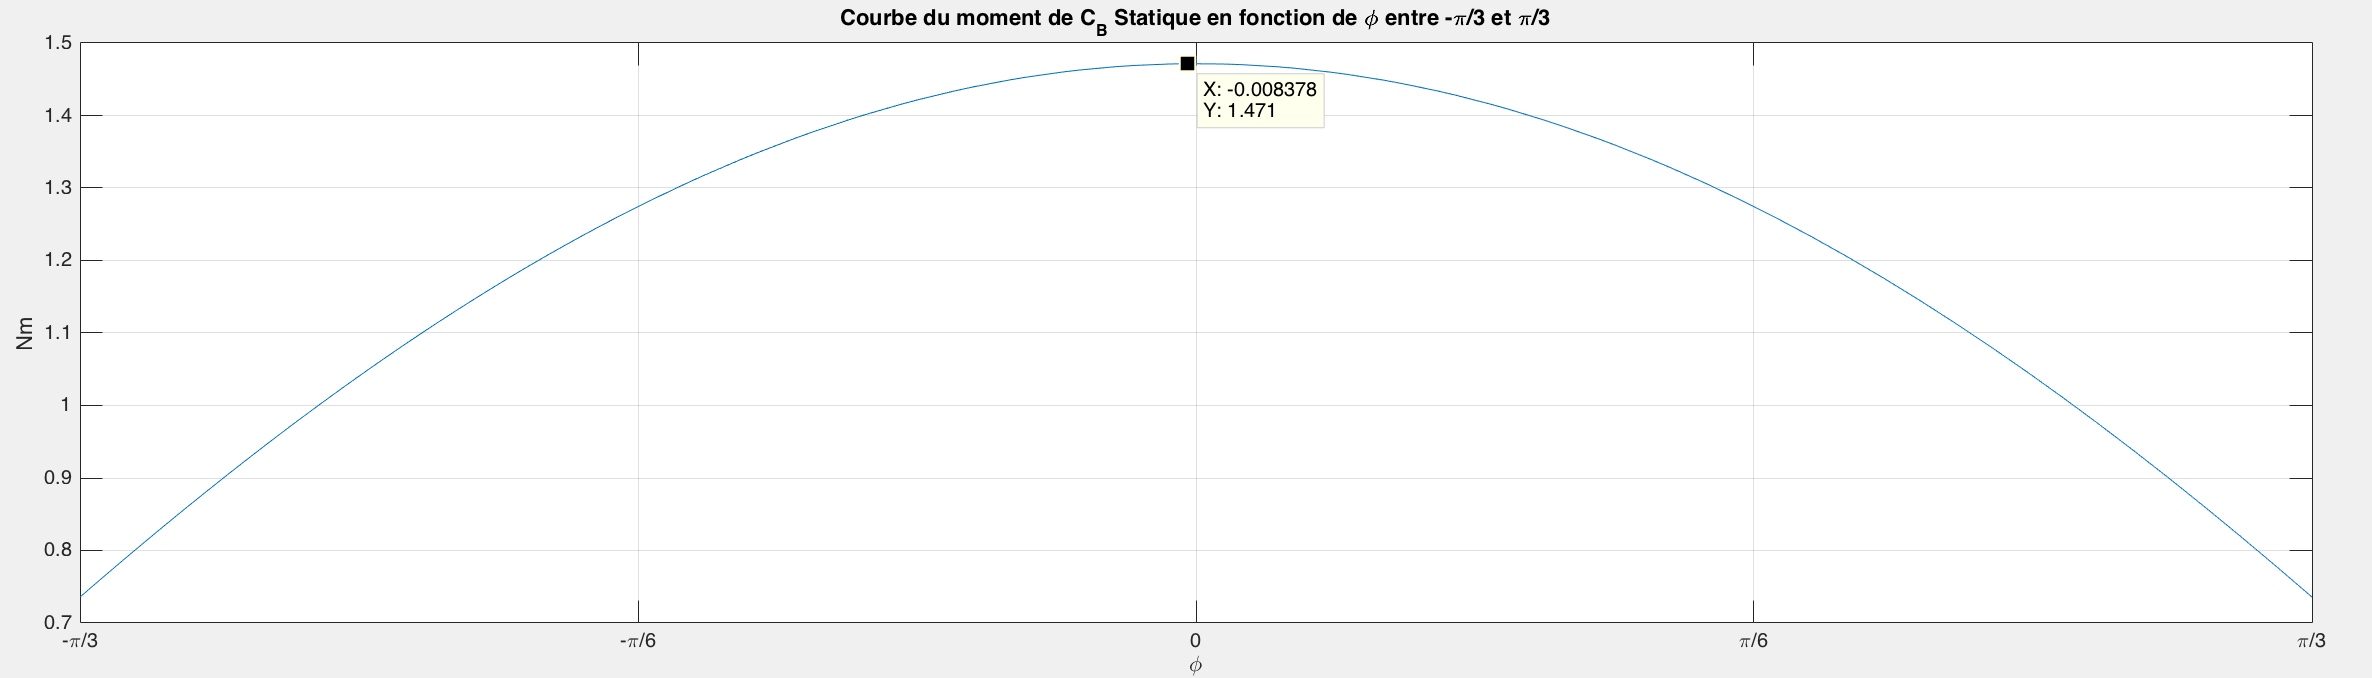
\includegraphics[width=\textwidth]{statique}
\newpage
\noindent Dynamique:
\newline
\noindent 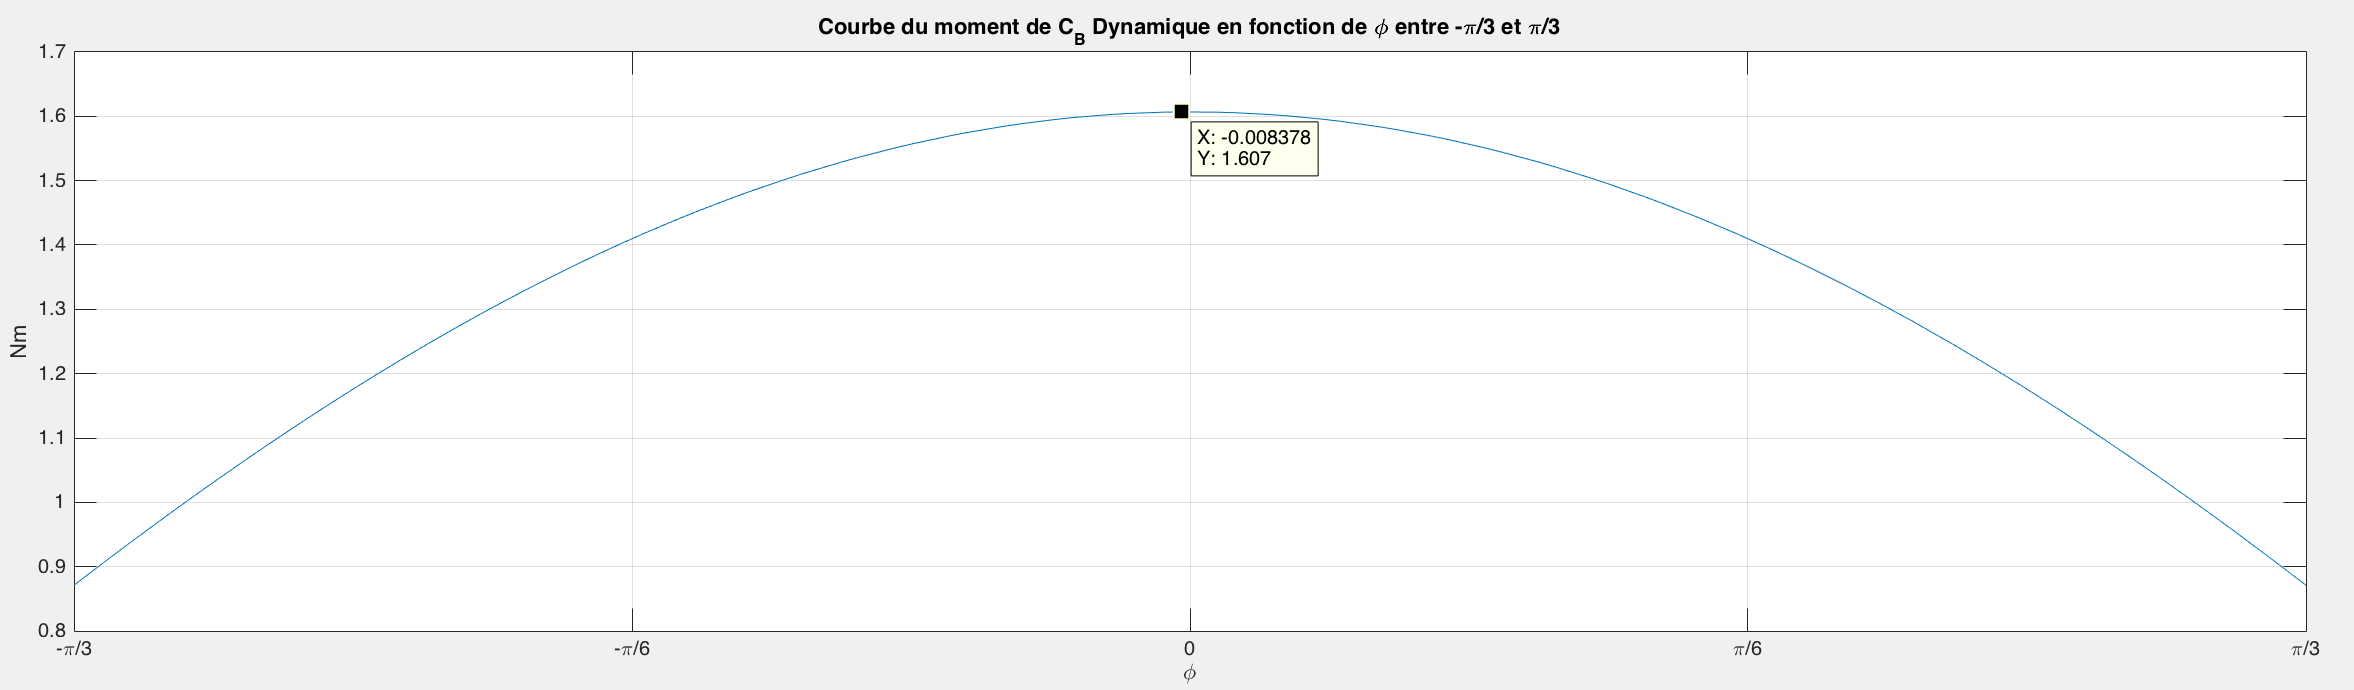
\includegraphics[width=\textwidth]{dynamique}

\subsubsection{Analyse des courbes de Statique et Dynamique}
\noindent
À première vue, on remarque que la courbe dynamique est plus élevée que la courbe statique. Cette observation est attendue, car afin de faire bouger un objet, il faut qu'il soit en équilibre (statique) et qu'on ajoute une force additionnelle. Il peut aussi être observé que la courbe dynamique semble représenter une simple translation positive sur l'axe des y de la courbe statique. Ce phénomène pourrait être expliqué par le fait qu'en statique, la somme des forces est égale à 0, mais qu'en dynamique, la somme des forces est non nulle. Cette différence entre la somme des forces en statique et dynamique semble représenter la valeur numérique de la translation de la courbe statique vers le courbe dynamique.

\section{Conclusion}
\noindent
Pour conclure, l'analyse des éléments physiques du robot, a permis de trouver une relation du point A dans le cas général, seulement sur le mouvement horizontal et seulement sur le mouvement vertical. De plus, à l'aide de cette relation, les courbes du cas horizontal et vertical ont permis de tracer les configurations initiales et finales du robot. L'analyse de l'analyse de l'équilibre du système a permis de trouver les forces lorsque robot est immobile et lorsqu'il est en mouvement. De ce, la force $\overrightarrow{F_B}$ a été trouvés et cette force a permis de trouver le couple $M_B$ du système a l'équilibre et lorsqu'il y a une force constant $\alpha$ appliquer au bras BA.
\end{document}
